\section{ARCHITECTURE DESIGN AND IMPLEMENTATION} 
\label{sec:architecture}
\subsection{Overall Architecture}

Our accelerator engine consists of multiple PE arrays connected to the off-chip memory via an AXI bus interface, as shown in Figure \ref{fig:overall_architecture}.
Each PE acts as one kernel and can take one S-W task to maximize throughput.

Before the accelerator starts to operate, the host processor assembles a set of query and target sequence pairs and streams them to the on-board DDR3 memory via PCIe. 
Then, each PE array's task distributor fetches a certain number of sequence pairs and distributes them to the idled PEs. 
The resulting mappings are stored in the on-board memory and then sent back to the host.
\subsection{Processing Element (PE) Design}
A PE realizes the S-W code obtained from the software implementation in BWA-MEM. 
We design our PE architecture using the high-level synthesis methodology. 
Unlike wavefront-based solutions which look completely different from the software approach,  
our design naturally follows the original software approach, which considerably shortens the development period. 

To maximize throughput, we make the initiation interval (II) be equal to 1 (II=1), i.e., calculating one cell of the score matrix per cycle. 
Moreover, a piece of conditional branch logic is implemented to realize pruning. 
It enlarges the size of each PE by 20\%, but reduces computation effort by over 50\%.  
%%%To maximize the throughput, we have to make the initiation interval (II) of the inner loop be equal to 1 (II=1). 
%%%To achieve ``II=1'', we propose the following microachitecture improvements. 
%%%First, we merge \textit{loop\_bounds\_update()} into the inner loop so that the update of \emph{beg} and \emph{end} 
%%%can be done in parallel with \textit{score\_calculation()}.
%%%Second, both the read and write operations of array \emph{e} and \emph{h} occur at the same cycle.
%%%The proposed solution is to realize the two arrays by using dual-port BRAM blocks
%%%and insert registers to guarantee that the read and write addresses are different.
%%%Listing \ref{list:ksw_extend2} shows the C kernel function, \textit{ksw\_extend2()}, 
%%%which contains a two-level nested loop to accomplish the alignment procedure.
%%%The two sequence arrays, \textit{query} and \textit{target}, are sent to the function as inputs.
%%%The other inputs are constants (\emph{o\_del}, \emph{e\_del}, \emph{o\_ins}, and \emph{e\_ins}) or the outputs from previous host functions (\emph{h0}).
%%%Array \emph{e} and \emph{h} are used to keep temporary scores.
%%%From a high-level point of view, the function is composed of four subfunctions: 
%%%(1) \textit{init()}, (2) \textit{score\_calculation()}, (3) \textit{loop\_bounds\_update()}, and (4) \textit{results\_generation()}.
%%%\textit{score\_calculation()} can fill one element in the score matrix
%%%while \textit{loop\_bounds\_update()} calculates the beginning point (\emph{beg}) and the ending point (\emph{end}) for the next iteration for pruning.
%%%
%%%
%%%%Figure \ref{fig:pe_archi} shows the architecture design of a PE.
%%%%The \emph{query} and \emph{target} arrays store the sequences of the input seed and the reference genome segment.
%%%%In the outer loop, the kernel traverses the \emph{target} array, where \emph{i} is the array index.
%%%%In the inner loop, the kernel traverses the \emph{query} array (index: \emph{j}) and fills all the elements successively in this column in the score matrix. 
%%%%A table lookup in the \textit{match table} is required to compute a temporary value (\emph{t}) for the current element. 
%%%%Moreover, the kernels also need to look up two more scores from the up-left and left neighbors, which have been computed in the previous outer-loop iteration.
%%%%These two scores of the two neighbors are saved in \emph{h}[\emph{j}] and \emph{e}[\emph{j}], respectively.
%%%%The score of the up neighbor is stored in register \emph{f}.
%%%%With \emph{t}, \emph{f}, \emph{h}[\emph{j}] and \emph{e}[\emph{j}], the score of the current position can be computed.
%%%
%%%We design our PE architecture by using the high-level synthesis methodology \cite{Cong2004}.
%%%Figure \ref{fig:pe_archi} shows the architecture design of a PE.
%%%To maximize the throughput, we have to make the initiation interval (II) of the inner loop be equal to 1 (II=1). 
%%%To achieve ``II=1'', we propose the following microachitecture improvements. 
%%%First, we merge \textit{loop\_bounds\_update()} into the inner loop so that the update of \emph{beg} and \emph{end} 
%%%can be done in parallel with \textit{score\_calculation()}.
%%%Second, both the read and write operations of array \emph{e} and \emph{h} occur at the same cycle.
%%%The proposed solution is to realize the two arrays by using dual-port BRAM blocks
%%%and insert registers to guarantee that the read and write addresses are different.
%%%
%%%\begin{lstlisting}[language={c++},basicstyle=\small,
%%%caption={The ksw\_extend2() in BWA-MEM: a high-level view.},
%%%captionpos=b,
%%%label={list:ksw_extend2}]
%%%void ksw_extend2(int qlen, uint8_t *query, 
%%%   int tlen, uint8_t *target, int o_del, 
%%%   int e_del, int o_ins, int e_ins, int h0, 
%%%   ...)
%%%{
%%%   ...
%%%
%%%   // outer loop
%%%   for(int i = 0; i < tlen; i++) {
%%%      init();
%%%      // inner loop
%%%      for(int j = beg; j < end; j++) {
%%%         // fill one element in score matrix
%%%         score_calculation(query[j],
%%%            o_del, e_del, o_ins, e_ins, 
%%%            h0, e, h, i, j, ...);
%%%      }
%%%      // perform pruning
%%%      loop_bounds_update(mj, h, &beg, &end);
%%%      results_generation(mj, m);
%%%   }
%%%   ..
%%%}
%%%\end{lstlisting}
%%%
%%%\begin{figure}[!hbt]
%%%\begin{center}
%%%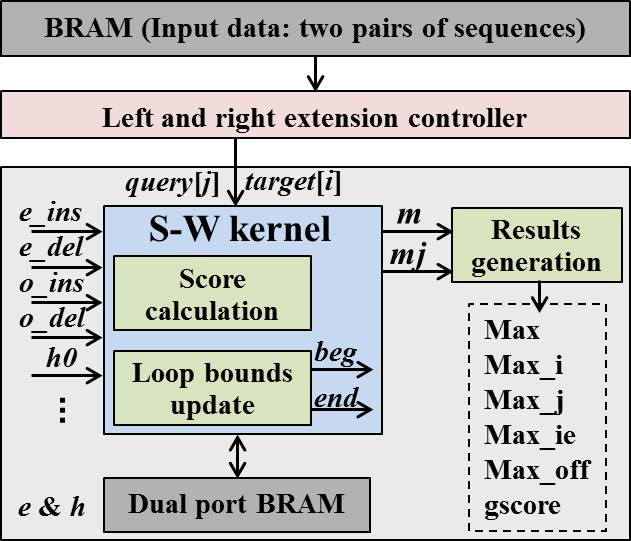
\includegraphics[width=2.8in]{Figures/Figure_Arch3.jpg}
%%%\caption {Architecture Design of a PE} \label{fig:pe_archi} \end{center} \end{figure}
%%%
%%%%First, the operation of reading BRAM data and the lookup in the \textit{match table} must complete in one clock cycle. 
%%%%Therefore, the \textit{match table} is implemented as individual registers. 
%%%%Second, both the read and write operations of array \emph{h} and \emph{e} occur at the same cycle. 
%%%%The proposed solution is to realize the two arrays by using dual-port BRAM blocks 
%%%%and insert registers to guarantee that the read and write addresses are different.
%%%
%%%Furthermore, since the extensions need to be performed in both ends of a seed,
%%%we merge both the left and right extention capability into our PE design and reuse the same S-W kernel, 
%%%as shown in Figure \ref{fig:pe_archi}.

\begin{figure}[!hbt]
\begin{center}
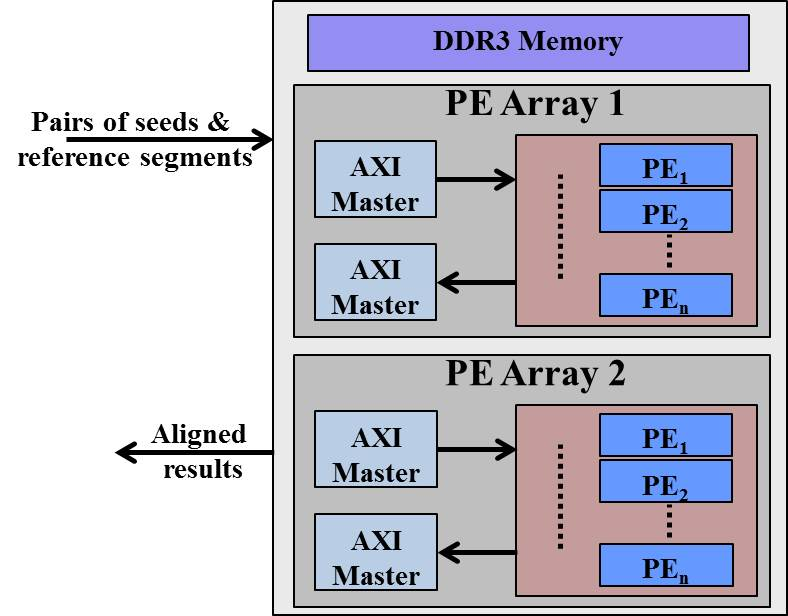
\includegraphics[width=2.5in]{Figures/Figure_Arch1.jpg}
\caption {Overall architecture of the proposed accelerator engine.} \label{fig:overall_architecture} \end{center} \end{figure}
\vspace{-10pt}

\subsection{Two-Level Task Scheduling}

The first level of task scheduling resides in a PE array. 
A PE array includes three types of major components: (1) \textit{task distributor}, (2) \textit{PE}, and (3) \textit{result collector}, 
as shown in Figure \ref{fig:schedule_structure}.
The \textit{task distributor} fetches data from the on-board DRAM to the on-chip BRAM and dynamically dispatches the tasks to each PE through a FIFO.
%%%A PE array contains a number of PEs to read data from their own FIFOs and process the S-W tasks in parallel.
The \textit{result collector} receives mapping results from each PE through a FIFO and packs them together for the host.

\begin{figure}[!hbt]
\begin{center}
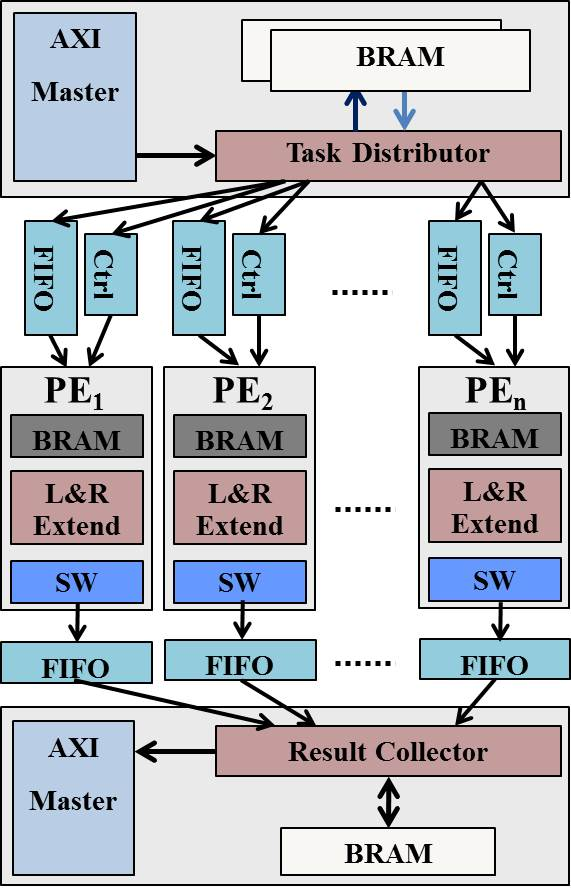
\includegraphics[width=2.5in]{Figures/Figure_Arch2.jpg}
\caption {The design of a PE array.} \label{fig:schedule_structure} \end{center} \end{figure}
\vspace{-10pt}


If a centralized \textit{task distributor} is not provided, each PE needs to fetch data from on-board memory independently. 
This incurs a significant (25\%) area overhead per PE to synthesize its own AXI interface. 
To reduce the overhead, we use only one AXI bus master for each \textit{task distributor} per PE array. 
The bus master fetches a group of data that meets the off-chip bandwidth demand of all PEs in the array. 
We also implement the ping-pong buffer operation by using double BRAM blocks for better performance. 
After the data are prefetched to BRAM, 
the distributor will check the flag of the FIFO of each PE one by one to find the available PEs. 
The \textit{task distributor} then transfers the S-W tasks from BRAM to the FIFOs of the available PEs. 
This process continues until all the tasks are processed.
The \textit{result collector} continues monitoring the output FIFO of each PE and obtaining results until all the results are received.

If the number of PEs is small, the first level of task scheduling is capable enough. 
However, when the number of PEs is increased to a certain point, 
the distributor becomes a performance bottleneck caused by its round-robin task scheduling manner.
Therefore, we explore the second level of task scheduling by replicating the number of PE arrays, i.e., the number of \textit{task distributors}. 
This two-level hierarchy provides us with a design methodology for obtaining scalable speedup with more PE arrays.
%%%
%%%
%%%%\subsection{High-level Synthesis Implementation}
%%%
%%%%All the above mentioned structures are described in C code and translated into RTL verilog code by the Vivado HLS tool. In addition, we take advantage of some special definitions and directives to guide the HLS tool to create the expected hardware architecture. For instance, the variable type of HLS stream is used to connect the three main parts with FIFOs (\ref{fig:pe_archi}). And the dataflow directive is utilized to make the parts run in parallel.
%%%
%%%%Derived from the benefit of high-level synthesis technique, the proposed architecture is easy to be adjusted for achieving scalability of acceleration, only by modifying a couple of parameters which define the number of duplication.
